\documentclass[11pt,a4paper]{article}
\usepackage{nabiadoc}
\usepackage{tikz}
\usetikzlibrary{positioning,arrows.meta,fit,calc}
\usepackage{caption}
\captionsetup[lstlisting]{justification=raggedright, singlelinecheck=false, font=small, labelfont=bf}
\usepackage{tabularx}

% Generated at build time by extract_snippets.py: excerpt locations, the MCP
% tool catalogue (tools.tex) and the AI configuration fields (config.tex).
\input{snippets.tex}
\newcommand{\snippetsource}[1]{\csname snippet@#1\endcsname}
\newcommand{\snippet}[3]{%
  \lstinputlisting[language=#2, caption={#3\\{\footnotesize\ttfamily\snippetsource{#1}}}]{#1.txt}}
% A prompt: plain text, wrapped.
\newcommand{\prompt}[2]{%
  \lstinputlisting[language={}, basicstyle=\ttfamily\scriptsize, keywordstyle={}, commentstyle={},
                   caption={#2\\{\footnotesize\ttfamily\snippetsource{#1}}}]{#1.txt}}
\lstset{basicstyle=\ttfamily\scriptsize, captionpos=t, numbers=none, aboveskip=8pt, belowskip=8pt,
        tabsize=4, keepspaces=true, breaklines=true, postbreak=\mbox{\textcolor{gray}{$\hookrightarrow$}\space}}
\renewcommand{\lstlistingname}{Code}
\newcommand{\sth}{\mathcal{S}}  % soft thresholding

% Pointers from a concept to its code.
\newcommand{\coderef}[1]{{\footnotesize\texttt{\snippetsource{#1}}}}
\newenvironment{codepointers}{%
  \par\smallskip\begingroup\footnotesize\noindent\textcolor{blue!50!black}{\textbf{Code}}\par\nopagebreak
  \begin{list}{}{\setlength{\leftmargin}{1.2em}\setlength{\itemsep}{0pt}\setlength{\parsep}{0pt}\setlength{\topsep}{1pt}}}%
  {\end{list}\endgroup\smallskip}
\newcommand{\codeitem}[2]{\item #2 --- \texttt{\snippetsource{#1}}}

% MCP tool catalogue entries (tools.tex).
\newcommand{\toolentry}[3]{\subsubsection*{\texttt{#1}}\vspace{-0.6em}
  \noindent{\footnotesize\textcolor{gray!30!black}{\emph{#2}\hfill\texttt{#3}}}\par\smallskip}
\newcommand{\modelentry}[2]{\subsubsection*{Input schema \texttt{#1}}\vspace{-0.6em}
  \noindent{\footnotesize\textcolor{gray!30!black}{\emph{pydantic model}\hfill\texttt{#2}}}\par\smallskip}
\newenvironment{toolparams}{\begin{description}\footnotesize\setlength{\itemsep}{0pt}\setlength{\parsep}{0pt}}{\end{description}}
% A reference to a section of another project's document.
\newcommand{\xref}[2]{\emph{#2} (#1 reference)}

\title{nabia web UI: Agents, MCP Servers and Web Application\\[0.3em]
\large Running the risk budgeting strategy with AI agents}
\author{nabia documentation}
\date{October 2026}

\begin{document}
\maketitle

\begin{abstract}
This document is the reference for the web UI project of nabia (\code{webui/}):
\begin{itemize}
  \item the AI layer: the three agents with their complete prompts, the MCP servers with
        every tool's description and input schema, the agent loop, how decisions become
        positions, and how news sentiment and relevance are produced and aggregated;
  \item the web application (FastAPI back end, JavaScript front end) and its job runner.
\end{itemize}
Every computation goes through the \code{nabia} package of the Python project, which runs the
C++ engines of the \code{nabia\_python\_bridge} wheel; their references are in
\code{python/doc} and \code{cpp/doc}. Excerpts, prompts, tool descriptions and configuration
fields are \emph{extracted from the source when the document is built}, so they are the text
the programs actually use.
\end{abstract}

\tableofcontents
\clearpage
%==============================================================================
\part{Overview}

\section{Purpose}
The web UI runs nabia's strategy day to day: agents read the news and the statistics, decide
the risk budgets, and the C++ engine turns them into positions; the web application starts
these jobs and shows every decision. The central design decision is to separate \emph{who
decides the risk budgets} from \emph{how budgets become positions}:
\begin{itemize}
  \item Budgets are decided by a fixed rule, by equal risk, or by AI agents.
  \item Positions come from a tested numerical engine (\code{nabia.latest\_weights} and
        \code{nabia.backtest}).
\end{itemize}
Agents never set weights. They choose budgets within bounds, and the engine computes the
weights, so an agent's influence is bounded and every decision is reproducible from its
stored budgets.

\section{Architecture}\label{sec:architecture}
\begin{figure}[ht]
\centering
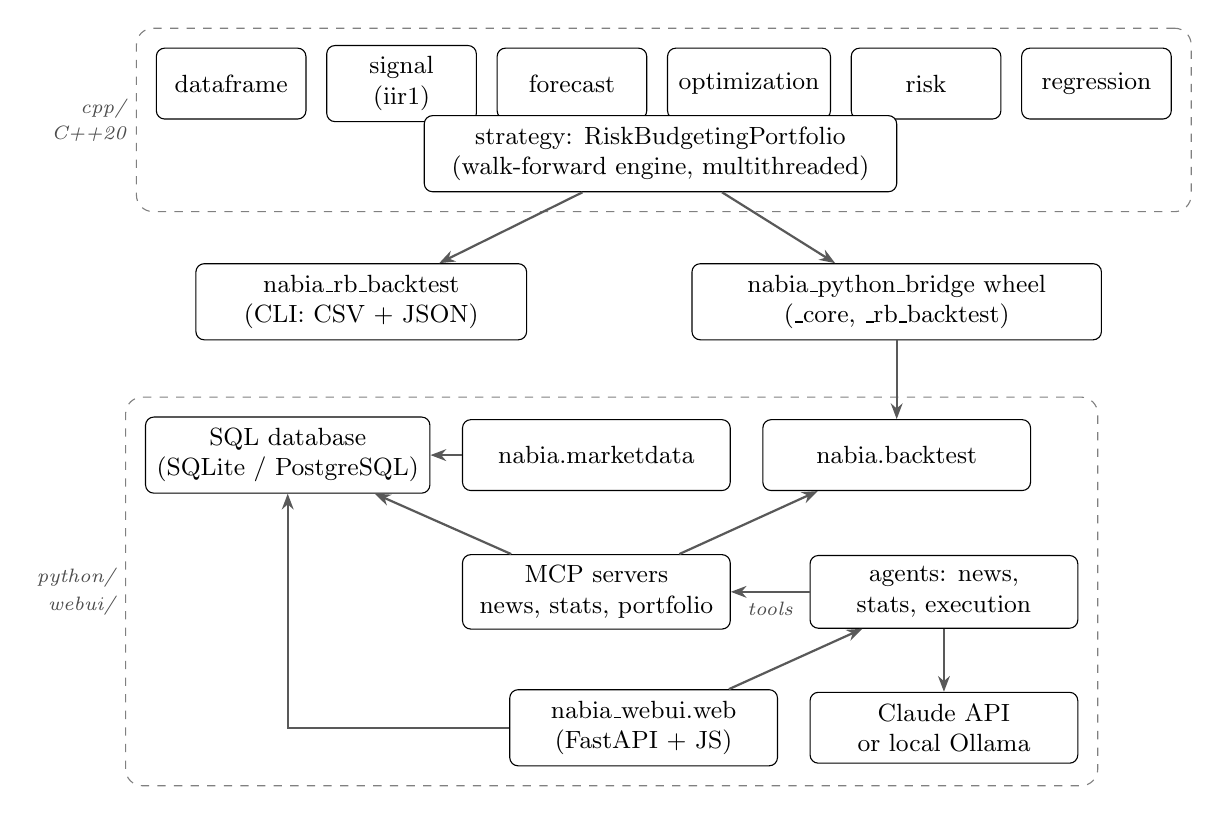
\begin{tikzpicture}[
  box/.style={draw, rounded corners=3pt, align=center, minimum height=9mm, font=\small, fill=white, inner sep=4pt},
  layer/.style={draw, dashed, rounded corners=6pt, inner sep=7pt, gray},
  arrow/.style={-{Stealth[length=2mm]}, thick, gray!70!black},
  lbl/.style={font=\scriptsize\itshape, gray!60!black}]
  \node[box, minimum width=19mm] (df) {dataframe};
  \node[box, right=2.5mm of df, minimum width=19mm] (sig) {signal\\(iir1)};
  \node[box, right=2.5mm of sig, minimum width=19mm] (fc) {forecast};
  \node[box, right=2.5mm of fc, minimum width=19mm] (opt) {optimization};
  \node[box, right=2.5mm of opt, minimum width=19mm] (risk) {risk};
  \node[box, right=2.5mm of risk, minimum width=19mm] (reg) {regression};
  \node[box, below=4mm of $(fc)!0.5!(opt)$, minimum width=60mm] (strat) {strategy: RiskBudgetingPortfolio\\(walk-forward engine, multithreaded)};
  \node[layer, fit=(df)(reg)(strat), label={[lbl]left:\shortstack[r]{cpp/\\C++20}}] (core) {};
  \node[box, below=9mm of strat, xshift=-38mm, minimum width=42mm] (cli) {nabia\_rb\_backtest\\(CLI: CSV + JSON)};
  \node[box, below=9mm of strat, xshift=30mm, minimum width=52mm] (bind) {nabia\_python\_bridge wheel\\(\_core, \_rb\_backtest)};
  \node[box, below=10mm of bind, minimum width=34mm] (pf) {nabia.backtest};
  \node[box, left=4mm of pf, minimum width=34mm] (md) {nabia.marketdata};
  \node[box, left=4mm of md, minimum width=30mm] (db) {SQL database\\(SQLite / PostgreSQL)};
  \node[box, below=8mm of md, minimum width=34mm] (mcp) {MCP servers\\news, stats, portfolio};
  \node[box, right=10mm of mcp, minimum width=34mm] (agents) {agents: news,\\stats, execution};
  \node[box, below=8mm of agents, minimum width=34mm] (llm) {Claude API\\or local Ollama};
  \node[box, left=4mm of llm, minimum width=34mm] (web) {nabia\_webui.web\\(FastAPI + JS)};
  \node[layer, fit=(db)(pf)(mcp)(agents)(llm)(web), label={[lbl]left:\shortstack[r]{python/\\webui/}}] (py) {};
  \draw[arrow] (strat) -- (cli);
  \draw[arrow] (strat) -- (bind);
  \draw[arrow] (bind) -- (pf);
  \draw[arrow] (md) -- (db);
  \draw[arrow] (mcp) -- (db);
  \draw[arrow] (mcp) -- (pf);
  \draw[arrow] (agents) -- node[lbl, below]{tools} (mcp);
  \draw[arrow] (agents) -- (llm);
  \draw[arrow] (web) -- (agents);
  \draw[arrow] (web.west) -| (db.south);
\end{tikzpicture}
\caption{The whole system and its three projects. Arrows point from a component to what it uses.}
\label{fig:architecture}
\end{figure}
\subsection{Three projects}
The repository holds three independent projects. Each opens on its own in an IDE, and each
has its own documentation in a \code{doc} folder:
\begin{center}\small
\begin{tabularx}{\linewidth}{@{}l l X@{}}
\toprule
Folder & IDE & Contents \\
\midrule
\code{cpp/} & CLion (CMake) & the C++ library (\code{include}, \code{src}), its tests, the
  command-line application, and the pybind11 bindings that build the
  \code{nabia\_python\_bridge} wheel into \code{dist/} \\
\code{python/} & PyCharm & the \code{nabia} package (backtests, analytics, market data) on top of
  the wheel, the examples, and the Python tests including the bridge tests \\
\code{webui/} & PyCharm & \code{nabia\_webui}: the agents, their MCP servers and the web app, on
  top of the \code{nabia} package \\
\bottomrule
\end{tabularx}
\end{center}
The projects depend on each other only through installed packages: \code{cpp} builds the wheel,
\code{python} installs it (\code{python/scripts/setup\_env.sh}), and \code{webui} installs both the
wheel and \code{python} in editable mode (\code{webui/scripts/setup\_env.sh}). Shared data, the market
database \code{data/market.db}, is at the repository root.

\subsection{Directory map}
\begin{center}\small
\begin{tabular}{@{}l>{\raggedright\arraybackslash}p{10cm}@{}}
\toprule
Path (in \code{webui/}) & Contents \\
\midrule
\code{nabia\_webui/ai/agents} & agent runtime, providers (Claude API, Ollama), the agent team \\
\code{nabia\_webui/ai/servers} & MCP servers: news, stats, portfolio \\
\code{nabia\_webui/ai} & configuration, database tables, pipeline (daily and backtest), command line \\
\code{nabia\_webui/web} & FastAPI back end (\code{app.py}), job runner, static front end \\
\code{tests} & pytest suites \\
\code{ai\_config.json} & configuration (symbols, bounds, model, database URL) \\
\code{scripts/setup\_env.sh} & creates \code{.venv} with the wheel, \code{nabia} and \code{nabia\_webui} \\
\code{doc} & this reference (LaTeX source, PDF, \code{build.sh}) \\
\bottomrule
\end{tabular}
\end{center}
One SQL database holds prices, news, statistics reports, decisions, agent transcripts, jobs,
job logs and backtest runs. Access goes through SQLAlchemy Core with portable types, so moving
from SQLite to PostgreSQL changes only the URL. By default it is the shared
\code{../data/market.db}.

\subsection{Environment}
\begin{lstlisting}[language=bash]
webui/scripts/setup_env.sh                                  # webui/.venv
cd webui && .venv/bin/python -m pytest                      # 24 tests, 1 opt-in (Ollama) skipped
.venv/bin/python -m nabia_webui.web --config ai_config.json   # http://127.0.0.1:8000
.venv/bin/python -m nabia_webui.ai daily --config ai_config.json
\end{lstlisting}
In PyCharm, open \code{webui/} and select \code{webui/.venv} as the interpreter; run
configurations should use \code{webui/} as the working directory, where \code{ai\_config.json}
and its relative database path resolve.

%==============================================================================
\part{The AI layer}

\section{Agents: roles, data flow and configuration}\label{sec:agents}



\begin{center}\small
\begin{tabularx}{\linewidth}{@{}l X X@{}}
\toprule
Agent & Tools & Output \\
\midrule
News analyzer & \code{news} server; on Claude also web search and web fetch & stored articles with topic, assets, sentiment, relevance \\
Stats analyzer & \code{stats} server & a structured report (\code{StatsReport}) with a budget tilt per asset \\
Execution agent & \code{news} and \code{stats} read-only, \code{portfolio} & risk budgets with a rationale, then target weights from the C++ engine \\
\bottomrule
\end{tabularx}
\end{center}

\begin{figure}[htbp]
\centering
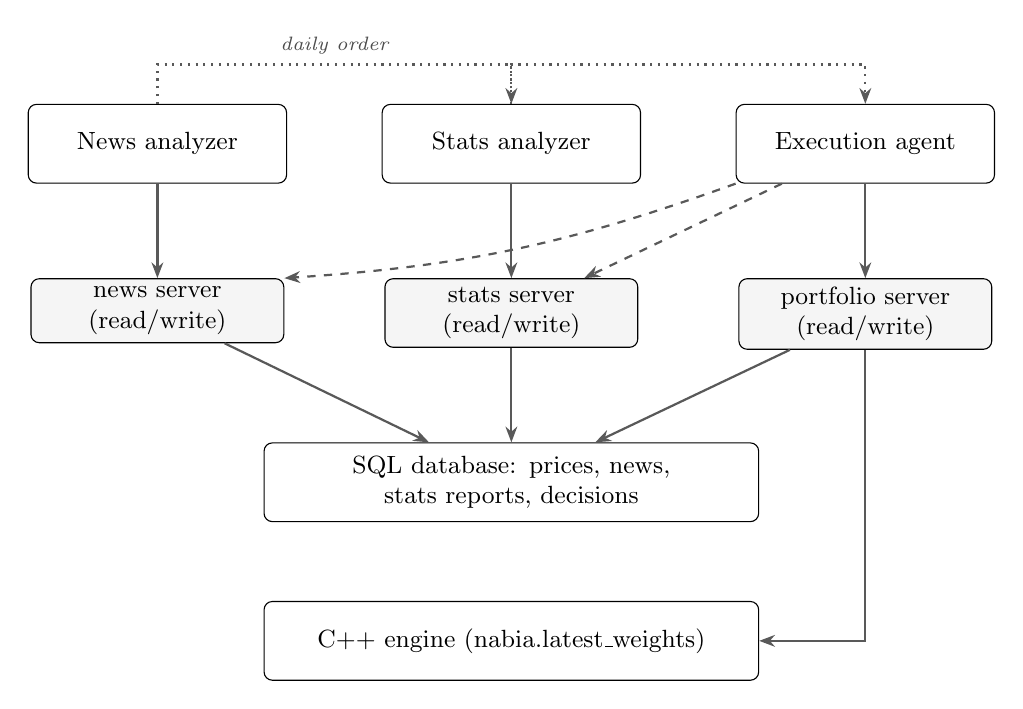
\begin{tikzpicture}[
  box/.style={draw, rounded corners=3pt, align=center, minimum height=10mm, font=\small, fill=white, inner sep=4pt, text width=30mm},
  srv/.style={draw, rounded corners=3pt, align=center, minimum height=8mm, font=\small, fill=gray!8, inner sep=3pt, text width=30mm},
  arrow/.style={-{Stealth[length=2mm]}, thick, gray!70!black},
  lbl/.style={font=\scriptsize\itshape, gray!60!black}]
  \node[box] (news) {News analyzer};
  \node[box, right=12mm of news] (stats) {Stats analyzer};
  \node[box, right=12mm of stats] (exec) {Execution agent};
  \node[srv, below=12mm of news] (sn) {\code{news} server\\(read/write)};
  \node[srv, below=12mm of stats] (ss) {\code{stats} server\\(read/write)};
  \node[srv, below=12mm of exec] (sp) {\code{portfolio} server\\(read/write)};
  \node[box, below=12mm of ss, text width=60mm] (db) {SQL database: prices, news, stats reports, decisions};
  \node[box, below=10mm of db, text width=60mm] (cpp) {C++ engine (\code{nabia.latest\_weights})};
  \draw[arrow] (news) -- (sn);
  \draw[arrow] (stats) -- (ss);
  \draw[arrow] (exec) -- (sp);
  \draw[arrow, dashed] (exec) -- (ss);
  \draw[arrow, dashed] (exec.south west) to[bend left=8] (sn.north east);
  \draw[arrow] (sn) -- (db);
  \draw[arrow] (ss) -- (db);
  \draw[arrow] (sp) -- (db);
  \draw[arrow] (sp.south) |- (cpp.east);
  \draw[arrow, dotted] (news.north) -- ++(0,5mm) -| node[lbl, above, pos=0.25]{daily order} (stats.north);
  \draw[arrow, dotted] (stats.north) -- ++(0,5mm) -| (exec.north);
\end{tikzpicture}
\caption{The three agents, the MCP servers they use, and their order in the daily pipeline. Dashed arrows: read-only access (the servers run with \code{-{}-read-only}).}
\label{fig:agents}
\end{figure}

\paragraph{Pipelines.}
\begin{itemize}
  \item The \emph{daily} pipeline runs news, then stats, then execution, for today.
  \item The \emph{backtest} pipeline runs stats and execution at each decision date
        (\S\ref{sec:backtest-mode}).
\end{itemize}
Every agent run is stored with its turns, tool calls (inputs and outputs, truncated to
2,000 characters), token usage and any error, which gives a complete audit trail.
\begin{codepointers}
  \codeitem{team_run}{running and recording an agent}
  \codeitem{run_daily}{daily pipeline}
  \codeitem{db_tables}{database tables}
\end{codepointers}

\subsection{Configuration}\label{sec:aiconfig}
Agents, servers and pipeline share one \code{AIConfig}, saved as JSON so that the MCP server
processes read the same settings. Unknown keys are rejected. Validation requires at least
two distinct symbols, $0<b_{\min}\le1/n\le b_{\max}\le1$, a known provider, and no
\code{budgets} in \code{portfolio}, because budgets are what the agents decide.
\begin{center}\footnotesize
\input{config.tex}
\end{center}
\begin{codepointers}
  \codeitem{ai_config}{\code{AIConfig}}
\end{codepointers}

\section{MCP servers and tool catalogue}\label{sec:tools}

\subsection{Design}
Each server is a standalone MCP server over stdio:
\begin{lstlisting}[language=bash]
python -m nabia_webui.ai.servers.<name> --config ... --run ... [--read-only]
\end{lstlisting}
The agents use them, and so can any MCP client, for example Claude Code. A server is built in three
layers:
\begin{itemize}
  \item A \code{ServerContext} holds the configuration, the run name and the two stores
        (market data and agent data).
  \item Tools are plain Python functions registered with \code{@tool(server)}.
  \item The MCP library derives each tool's \emph{description} from the function's
        docstring and its \emph{input schema} from the type annotations. The catalogue
        below is extracted from the same source, so it is exactly what the model sees.
\end{itemize}

Four rules apply to every tool.
\begin{description}
  \item[Point in time] Analytical tools take \code{as\_of} (\code{YYYY-MM-DD}) and read only
        data dated on or before it. A test rewrites every price after \code{as\_of} and
        checks that every tool's output is unchanged.
  \item[Errors the model can act on] Anticipated failures, such as wrong symbols or
        out-of-range values, raise \code{ValueError} or \code{KeyError}. The decorator turns
        them into MCP \code{ToolError}s carrying the message, so the model sees why a call
        failed and can correct it. Any other exception would reach the model only as a
        generic error.
  \item[Read-only mode] \code{-{}-read-only} omits the tools that write. The execution agent
        cannot store news or overwrite statistics reports.
  \item[Runs] \code{-{}-run <name>} scopes reports and decisions to a backtest run, or to
        \code{live}, so backtests never mix with live decisions.
\end{description}
\snippet{tool_decorator}{Python}{Tool registration}
\snippet{parse_as_of}{Python}{The as-of date}
\begin{codepointers}
  \codeitem{server_context}{\code{ServerContext}}
  \codeitem{server_prices}{prices up to as\_of, universe check}
  \codeitem{clean}{JSON cleaning (NaN to null, rounding)}
  \codeitem{news_server}{news server}
  \codeitem{stats_server}{stats server}
  \codeitem{portfolio_server}{portfolio server}
\end{codepointers}

\subsection{Catalogue}
The rest of this section is generated from the server sources. For each tool it gives the
description shown to the model, whether the tool writes, the source location, and the
parameters with their types and defaults. The input schemas of the structured tools follow
each server. In the news schemas, \code{Topic} is one of:
\begin{itemize}
  \item monetary\_policy, inflation, growth, labor, earnings, fiscal, geopolitics;
  \item energy, metals, agriculture, crypto, rates, credit, fx, regulation, other.
\end{itemize}
\code{AssetClass} is one of equity\_index, bond\_future, commodity and crypto.

\input{tools.tex}

\section{The agent runtime}\label{sec:runtime}

\subsection{Starting an agent}
\code{AgentRuntime.run} starts the agent's MCP servers as subprocesses. They use the same
Python interpreter and module path, with \code{-{}-config} pointing to the saved
configuration and \code{-{}-run} set to the run name. The runtime then:
\begin{itemize}
  \item initializes a client session per server;
  \item lists the tools of every session and rejects name collisions between servers;
  \item adds the hosted tools, if any (web search and fetch on Claude);
  \item runs the loop.
\end{itemize}
Errors raised inside the loop are re-raised only after the sessions close cleanly.
Otherwise the MCP task groups would wrap them in an \code{ExceptionGroup}.
\begin{codepointers}
  \codeitem{runtime_run}{run: servers, tools, loop}
  \codeitem{server_parameters}{server subprocess parameters}
  \codeitem{runtime_client}{client selection by provider}
\end{codepointers}

\subsection{The loop}
The runtime uses a manual tool-use loop, not an SDK tool runner. One agent talks to several
MCP processes at once, mixes their tools with hosted tools, and records every call. Each
turn proceeds as follows.
\begin{enumerate}
  \item \textbf{Request.} One request carries the system prompt, the tools and the
        conversation so far, plus these options:
        \begin{itemize}
          \item \code{max\_tokens}: 16,000;
          \item adaptive thinking;
          \item the agent's effort level;
          \item prompt caching of the stable prefix (tools, system prompt, history);
          \item server-side refusal fallbacks.
        \end{itemize}
  \item \textbf{Streaming.} The reply is \emph{streamed}. Text and thinking deltas go to
        the log as they arrive, so a job's log follows the model live (\S\ref{sec:web}).
  \item \textbf{Stop reasons.}
        \begin{itemize}
          \item \code{refusal} raises an error naming the category.
          \item \code{pause\_turn} (a long hosted-tool turn) resends the conversation so
                the model can resume.
          \item \code{max\_tokens} is an error.
          \item Any other reason that is not \code{tool\_use} ends the run with the final
                text.
        \end{itemize}
  \item \textbf{Tools.} All \code{tool\_use} blocks of the turn run concurrently. Their
        results return \emph{in one user message}. A failing tool, or a crashed server,
        becomes an error result, so the agent can recover.
\end{enumerate}
A run is limited to 40 turns.
\snippet{runtime_loop}{Python}{The agent loop}
\snippet{runtime_create}{Python}{One streamed model turn}
\snippet{live_output}{Python}{Live logging of streamed output}
\snippet{runtime_call_tool}{Python}{Executing one tool call on its MCP server}

\subsection{Providers}
\begin{description}
  \item[Claude] (\code{provider: "anthropic"}) uses \code{claude-opus-5-5} through the
        Anthropic SDK with the options above.
  \item[Local model] (\code{provider: "ollama"}) uses an adapter that exposes the same
        interface (\code{beta.messages.create} and \code{.stream}) and translates to
        Ollama's chat API:
        \begin{itemize}
          \item the system prompt becomes a system message, and tools become function tools;
          \item assistant \code{tool\_use} blocks become \code{tool\_calls}, and
                \code{tool\_result} blocks become \code{tool} messages (errors prefixed
                \code{ERROR:});
          \item streamed NDJSON chunks become text and thinking deltas, and the merged
                reply becomes the final message;
          \item Claude-only options are ignored, and hosted tools are dropped, so local
                news comes from RSS.
        \end{itemize}
        Model options (temperature 0.2, a 32k context) come from the configuration.
\end{description}
\snippet{ollama_stream}{Python}{Ollama streaming as Anthropic-style events}
\snippet{ollama_response}{Python}{Ollama replies translated to content blocks}
\begin{codepointers}
  \codeitem{ollama_messages}{request translation}
  \codeitem{ollama_chat}{HTTP call, streamed or not}
\end{codepointers}

\section{Agent prompts}\label{sec:prompts}

\subsection{Structure and templating}
Every system prompt has the same five parts:
\begin{enumerate}
  \item the agent's role in a cross-asset trend portfolio;
  \item the \emph{as-of rule};
  \item the portfolio universe;
  \item the job;
  \item a numbered workflow that names the tools to use, ending with the expected output.
\end{enumerate}
\code{AgentTeam.\_fill} fills the templates:
\begin{description}
  \item[\code{\{as\_of\}}] the decision date. In live mode it is today.
  \item[\code{\{universe\}}] one line per portfolio symbol, \code{- SYMBOL: name, asset\_class},
        from the asset table.
  \item[\code{\{as\_of\_rule\}}] the rule below, with the date filled in.
  \item[\code{\{news\_days\}}] the news window of the execution agent (7 by default).
  \item[\code{\{research\}}] the news analyzer's research step. With web access (Claude) it
        adds web search and fetch. With a local model it uses the RSS headlines only.
  \item[\code{\{mode\_note\}}] the backtest note for non-live runs, and empty otherwise.
\end{description}
\prompt{as_of_rule}{The as-of rule (in every system prompt)}
\snippet{team_fill}{Python}{Template filling}
\begin{codepointers}
  \codeitem{team_universe}{the universe lines}
\end{codepointers}

\subsection{News analyzer}
The news analyzer runs with effort \code{medium}, the \code{news} server (writable) and, on
Claude, web search and web fetch (each capped at \code{news\_max\_searches} uses). Its user
message is \emph{``Collect and store the market-moving news for \{as\_of\}.''} The prompt
defines the sentiment and relevance rubric (\S\ref{sec:sentiment}) and requires real URLs
and dates.
\prompt{news_system}{News analyzer system prompt (template)}

\subsection{Stats analyzer}
The stats analyzer runs with effort \code{high} and the \code{stats} server (writable). Its
user message is \emph{``Analyze the portfolio assets as of \{as\_of\} and save the stats
report.''} It must:
\begin{itemize}
  \item judge each asset's trend, volatility regime and diversification;
  \item propose a tilt in $[-1,1]$ proportionate to the evidence;
  \item save a schema-validated report (\code{StatsReport}) covering every symbol.
\end{itemize}
\prompt{stats_system}{Stats analyzer system prompt (template)}

\subsection{Execution agent}
The execution agent runs with effort \code{high}, the \code{news} and \code{stats} servers
read-only, and the \code{portfolio} server. Its user message is \emph{``Decide the risk
budgets for \{as\_of\} and compute the target weights.''} The prompt fixes its decision
policy:
\begin{itemize}
  \item start from equal risk;
  \item tilt mainly on the statistical evidence, using news as a secondary input;
  \item respect the bounds;
  \item keep budgets close to the previous decision because trading costs money, and
        explain any large change.
\end{itemize}
\prompt{execution_system}{Execution agent system prompt (template)}
\prompt{backtest_note}{Backtest note, appended for non-live runs (\code{\{mode\_note\}})}
\snippet{team_calls}{Python}{How each agent is called: prompts, user messages, servers, effort}

\section{From decisions to positions}\label{sec:decisions}

\subsection{Budget normalization within bounds}
The execution agent proposes positive \emph{relative} budgets $\tilde b$. The tool
\code{set\_risk\_budgets} maps them to budgets with $\sum_ib_i=1$ and
$b_{\min}\le b_i\le b_{\max}$:
\begin{enumerate}
  \item Let $F$ be the set of fixed assets, initially empty. Scale the free assets to fill
        the rest: $b_i=\tilde b_i\,(1-\sum_{j\in F}b_j)/\sum_{j\notin F}\tilde b_j$.
  \item Fix every free asset below $b_{\min}$ at $b_{\min}$, and every one above $b_{\max}$
        at $b_{\max}$.
  \item Repeat until nothing is out of bounds. If every asset ends fixed, renormalize the
        fixed values.
\end{enumerate}
This is well defined whenever $nb_{\min}\le1\le nb_{\max}$, which validation guarantees.
Each pass fixes at least one asset, so it ends after at most $n$ passes. The free assets
keep their proposed \emph{ratios}, so the rule changes the agent's intent as little as the
bounds allow.

The tool returns the budgets and how far the bounds moved each one. \code{preview\_budgets}
shows the same result without saving it.
\snippet{project_budgets}{Python}{Budget normalization}
\snippet{set_risk_budgets}{Python}{The decision tool}

\subsection{Target weights}
\code{compute\_target\_weights} loads at least
$\max(3W+30,\,120)$ calendar days of prices up to \code{as\_of}. It runs
\code{nabia.latest\_weights} with the decided budgets, which is the engine of
\xref{C++}{The walk-forward portfolio engine} restricted to the last rebalance. It stores the weights and leverage
with the decision.

Each decision records who made it, as \code{trend\_rule} or as
\code{agent:<model>} (for example \code{agent:ollama:qwen3.8:latest}). Runs on different
models can therefore be compared.
\snippet{compute_weights}{Python}{Budgets to target weights through the C++ engine}

\subsection{The trend rule baseline}
A transparent, model-free policy is the benchmark that agent policies must beat:
\[
  \tilde b_i=\max\!\big(1+s\cdot\mathrm{clip}(m_i,-1,1),\,10^{-6}\big),\qquad s=0.5,
\]
followed by the same bounded normalization. A missing momentum counts as 0. A strong
uptrend ($m_i\ge1$) gets $1.5\times$ the equal budget before normalization, and a strong
downtrend $0.5\times$. Over 2019--2026, on the default universe with monthly decisions, it
reached a Sharpe ratio of 0.96 against 0.92 for equal risk.
\snippet{trend_tilted_budgets}{Python}{The trend rule}
\begin{codepointers}
  \codeitem{trend_rule_decider}{trend rule as a backtest policy}
\end{codepointers}

\subsection{Backtest mode}\label{sec:backtest-mode}
\paragraph{Decision dates.} The trading dates in $[\text{start},\text{end}]$: every one for
\code{D}, or the last of each week (\code{W-FRI}), month (\code{ME}) or quarter (\code{QE}).

\paragraph{Policies.}
\begin{itemize}
  \item \code{trend\_rule};
  \item \code{ollama} (agents on the local model);
  \item \code{claude} (agents on Claude);
  \item \code{agents} (agents on the configured provider).
\end{itemize}

\paragraph{Procedure.}
\begin{enumerate}
  \item At each date $d$, the policy decides budgets as of $d$. A date that already has a
        decision is skipped, so interrupted backtests resume.
  \item The decisions form a budget schedule. Budgets decided at the close of $d$ apply
        from the rebalance at $d$ on.
  \item One continuous backtest runs with the schedule, together with an equal-risk
        baseline over the same period. The run's policy, period and metrics are stored.
\end{enumerate}
The decision frequency is not the trading frequency: trades follow the parameter
\code{rebalance\_frequency}, and each rebalance uses the latest decision.
\snippet{decision_dates}{Python}{Decision dates}
\snippet{evaluate_decisions}{Python}{Decisions to a backtest, against equal risk}
\begin{codepointers}
  \codeitem{run_backtest}{the backtest loop}
  \codeitem{make_decider}{policy to decider}
  \codeitem{agent_decider}{agent policy (stats, then execution)}
\end{codepointers}

\paragraph{Look-ahead control.} The tools cannot see the future. In backtests, news comes
only from the database (no web access), and the prompt asks the model to treat the decision
date as today. One leak cannot be closed by tooling: the language model was trained on data
up to its knowledge cutoff and may recognize market history before it. Agent backtests
inside that window are therefore optimistic. They are fully out of sample only after the
cutoff.

\section{News: collection, sentiment and relevance}\label{sec:sentiment}

\subsection{Collection}\label{sec:news-collection}
The news analyzer runs once a day in live mode.
\begin{enumerate}
  \item It calls \code{query\_news} for the last two days to see what is already stored.
  \item It gathers candidate stories.
        \begin{itemize}
          \item \code{fetch\_news\_feeds} reads ten public feeds: MarketWatch, CNBC (two),
                Financial Times, Investing.com, CoinDesk, OilPrice, the Federal Reserve, the
                ECB and the Bank of England. The list is configurable. The tool parses RSS
                and Atom, keeps items newer than \code{max\_age\_days}, removes URLs already
                stored, and returns the newest first, with HTML stripped from descriptions.
                A broken feed is reported without hiding the others.
          \item On Claude, web search and fetch also fill gaps and confirm stories.
        \end{itemize}
  \item It keeps 8--20 material stories, classifies them, and stores them with
        \code{store\_news\_articles}, keyed by URL (an upsert).
\end{enumerate}
\snippet{fetch_news_feeds}{Python}{RSS and Atom headlines without stored articles}
\begin{codepointers}
  \codeitem{read_feed}{feed parsing}
\end{codepointers}

\subsection{How sentiment and relevance are produced}
\textbf{Sentiment and relevance are judgements made by the language model for each article.
They are not computed by a statistical model or a word list.} The news analyzer reads the
headline and description, and on Claude possibly the article, then fills the
\code{NewsArticle} schema following the rubric in its prompt:
\begin{description}
  \item[Sentiment] $s\in[-1,1]$ is the \emph{expected price impact on the affected assets}:
        $-1$ clearly bearish, $+1$ clearly bullish, $0$ neutral or mixed. It is relative to
        the assets the story moves, not the tone of the text. A hawkish central bank is
        bearish for bonds even when the article reads upbeat.
  \item[Relevance] $r\in[0,1]$ is the importance of the story for a cross-asset
        portfolio: 1 for portfolio-wide shocks, about 0.5 for a story that moves one asset
        class, and lower for minor items.
  \item[Classification] covers the main topic, the affected asset classes, and the
        portfolio symbols directly affected.
\end{description}
The server validates what the model produces before storing it:
\begin{itemize}
  \item the schema bounds $s\in[-1,1]$ and $r\in[0,1]$;
  \item topic and asset classes from fixed lists;
  \item no future dates;
  \item symbols from the universe.
\end{itemize}
Invalid articles are rejected with a reason the model can act on.
\snippet{news_article}{Python}{Article schema}
\snippet{store_news_articles}{Python}{Validation before storage}

\subsection{Aggregation}
\code{news\_summary} takes the articles $A$ published in the $d$ days up to and including
\code{as\_of} and groups them by topic, asset class and symbol. An article that affects
several classes or symbols counts in each of their groups. For each group $g$ it reports:
\begin{itemize}
  \item the count;
  \item the maximum relevance;
  \item the \textbf{relevance-weighted sentiment}
\[
  S_g=\frac{\sum_{i\in g}s_i\,r_i}{\sum_{i\in g}r_i}.
\]
\end{itemize}
When all relevances in a group are zero, the denominator is replaced by 1, so $S_g=0$.
$S_g$ is a convex combination of the sentiments, so $S_g\in[-1,1]$. Weighting by relevance
lets one portfolio-wide story outweigh several minor ones. The summary also lists the ten
most relevant headlines.

The web application's \emph{News} page shows, over the selected filter, article counts per
day and the simple (unweighted) average sentiment per topic.
\snippet{news_summary}{Python}{Relevance-weighted aggregation}
\begin{codepointers}
  \codeitem{query_news}{article queries}
  \codeitem{store_news}{storage (upsert by URL)}
  \codeitem{web_news}{web News aggregates}
\end{codepointers}

\subsection{Use and limitations}
News is a \emph{secondary} input by design. The execution agent tilts mainly on statistics
and uses news to confirm, temper or flag risks the statistics do not show yet. Because the
scores are model judgements:
\begin{itemize}
  \item \textbf{They are not reproducible across models}, and only approximately across
        runs. Decisions record the model that made them.
  \item \textbf{They are uncalibrated.} A sentiment of $0.6$ has no defined relation to a
        return. Using them as quantitative signals would require calibration first, for
        example a regression of next-day returns on $S_g$.
  \item \textbf{Coverage depends on the sources.} RSS headlines and descriptions are short,
        and web access gives fuller context.
\end{itemize}
Possible improvements:
\begin{itemize}
  \item an ensemble of scoring models;
  \item a lexicon or finance-tuned classifier as a reproducible baseline;
  \item a calibration study of $S_g$ against returns.
\end{itemize}

%==============================================================================
\part{Operation}

\section{Web application and job runner}\label{sec:web}

\code{nabia\_webui.web} is a FastAPI application with a single-page JavaScript front end
(Chart.js). Start it with
\code{python -m nabia\_webui.web -{}-config ai\_config.json}; it binds to
127.0.0.1 by default.
\begin{center}\small
\begin{tabularx}{\linewidth}{@{}l X@{}}
\toprule
Endpoint & Purpose \\
\midrule
\code{GET /api/overview} & latest live decision, data coverage, recent jobs, model \\
\code{GET /api/news} & articles with filters, counts per day, sentiment by topic \\
\code{GET /api/runs}, \code{/api/runs/\{run\}/decisions} & runs and their decisions \\
\code{GET /api/runs/\{run\}/stats\_report} & a run's stats report as of a date \\
\code{GET /api/agent\_runs}, \code{/api/agent\_runs/\{id\}} & agent transcripts (tool calls, usage) \\
\code{GET /api/backtests/\{run\}} & equity, drawdown, metrics, schedule, weights vs equal risk \\
\code{GET /api/jobs}, \code{/api/jobs/\{id\}} & jobs and their status \\
\code{GET /api/jobs/\{id\}/logs?after=} & job log lines after a given id (tailing) \\
\code{POST /api/jobs} & start a job: \code{download}, \code{news}, \code{daily}, \code{backtest} \\
\bottomrule
\end{tabularx}
\end{center}

\paragraph{Jobs.} Jobs run one at a time, in order, in the server's event loop. SQLite
allows one writer, and agent runs are costly. Their status is stored in the database.
Blocking work runs in worker threads so the server stays responsive:
\begin{itemize}
  \item downloads;
  \item the trend rule;
  \item the final C++ backtest.
\end{itemize}

\paragraph{Live logs.} A logging handler stores every record emitted while a job runs,
under that job's id. The id lives in a \emph{context variable}, which follows the job into
its asyncio tasks and worker threads, so concurrent web requests never leak into a job's
log. The log therefore contains:
\begin{itemize}
  \item the pipeline's steps;
  \item each agent turn and each tool call, with input and output previews;
  \item the model's text and thinking as it streams. Long lines arrive in pieces of about
        400 characters, and slow streams every few seconds.
\end{itemize}
Chatty libraries contribute only warnings and errors. While the job runs, the front end
asks every second for the lines after the last one it has, and shows the model's streamed
text and thinking in their own styles.
\snippet{job_log_handler}{Python}{Per-job log capture}
\snippet{job_run}{Python}{Running a job with its log context}
\begin{codepointers}
  \codeitem{web_app}{application and endpoints}
  \codeitem{job_runner}{job runner}
  \codeitem{job_backtest}{backtest job}
  \codeitem{log_viewer}{front-end log viewer}
\end{codepointers}


\section{Verification}\label{sec:verification}
\begin{description}
  \item[pytest] (24 tests, offline by default):
        \begin{itemize}
          \item the three MCP servers in process (including the no-look-ahead check);
          \item the agent loop over real stdio MCP servers with a scripted model (parallel
                calls, tool errors, paused turns, refusals);
          \item the Ollama translation and streaming against a mock transport, and live
                log chunking;
          \item RSS parsing, the pipeline, and the web API with job logs.
        \end{itemize}
        An opt-in test (\code{NABIA\_OLLAMA\_TESTS=1}) runs the execution agent end to end on a
        local model. The analytics the servers use are tested in the Python project.
  \item[This document] Its excerpts, prompts, tool catalogue and configuration table are
        extracted at build time. A listed function that no longer exists stops the build.
\end{description}

\section{Limitations and future work}\label{sec:limitations}
\begin{itemize}
  \item \textbf{News scores} are uncalibrated model judgements (\S\ref{sec:sentiment}).
  \item \textbf{Agent backtests} before the model's knowledge cutoff are optimistic.
  \item \textbf{Jobs} run sequentially. A queue with a PostgreSQL backend would allow
        concurrent jobs.
\end{itemize}

\end{document}
